% ==============================================================================
% RapidBoxForest (RBF) - IEEE Transactions on Robotics submission source (EN).
% Submission-polished writing revision: improves terminology, claim alignment,
% and experimental accounting without adding new data or figures.
% Standalone-compilable from paper/ while reusing generated assets and figures
% from paper/generated/ and paper/figures/.
% ==============================================================================
% Load the silence package as early as possible to filter benign font warnings
% that are emitted during package/class loading in automated builds.
\RequirePackage{silence}
\WarningFilter{latexfont}{Font shape}
\WarningFilter{latexfont}{Some font shapes were not available}
\documentclass[journal]{IEEEtran}

% Font setup: keep the source portable across IEEE-style pdfLaTeX builds and
% XeLaTeX/LuaLaTeX builds.  For Unicode engines, load Latin Modern from TeX Live
% font files rather than relying on operating-system font discovery.
\usepackage{iftex}
\ifPDFTeX
  \usepackage[T1]{fontenc}
  \usepackage{lmodern}
\else
  \usepackage{fontspec}
  \setmainfont{lmroman10}[
    Extension=.otf,
    UprightFont=*-regular,
    BoldFont=*-bold,
    ItalicFont=*-italic,
    BoldItalicFont=*-bolditalic,
    Ligatures=TeX,
    Scale=MatchLowercase]
  \setsansfont{lmsans10}[
    Extension=.otf,
    UprightFont=*-regular,
    BoldFont=*-bold,
    ItalicFont=*-oblique,
    BoldItalicFont=*-boldoblique,
    Scale=MatchLowercase]
  \setmonofont{lmmono10}[
    Extension=.otf,
    UprightFont=*-regular,
    ItalicFont=*-italic,
    Scale=MatchLowercase]
\fi

% Loosen paragraph tolerance slightly to avoid underfull hbox warnings in
% narrow IEEE two-column layout while keeping good justification.
\tolerance=2000
\emergencystretch=2em
% Retain IEEEtran float and caption spacing defaults. Page fitting should come
% from text consolidation or supplementary material rather than global compression.

\usepackage{amsmath,amssymb,amsfonts}
\usepackage{amsthm}
\usepackage{algorithm}
\usepackage{algorithmic}
\usepackage{booktabs}
\usepackage{array}
\usepackage{graphicx}
\usepackage{tikz}
\usepackage{pgfplots}
\pgfplotsset{compat=1.18}
\usetikzlibrary{positioning,arrows.meta}
\usepackage{capt-of}
\usepackage{placeins}
\usepackage{bm}
\usepackage{cite}
\usepackage{hyperref}
\hypersetup{hidelinks}
\usepackage{cleveref}
\usepackage[inline]{enumitem}

\newtheorem{theorem}{Theorem}
\newtheorem{proposition}{Proposition}
\newtheorem{definition}{Definition}
\newtheorem{remark}{Remark}
\newtheorem{lemma}{Lemma}
\newtheorem{corollary}{Corollary}
\newtheorem{assumption}{Assumption}

\newcommand{\rbf}{RBF}
\newcommand{\iAABB}{\ensuremath{\mathrm{iAABB}}}
\newcommand{\Real}{\ensuremath{\mathbb{R}}}
\newcommand{\Ball}{\ensuremath{\mathbb{B}}}
\newcommand{\Cfree}{\ensuremath{\mathcal{C}_{\mathrm{free}}}}
\newcommand{\calO}{\ensuremath{\mathcal{O}}}
\newcommand{\Q}{\ensuremath{\mathcal{Q}}}
\newcommand{\cspace}{\mbox{C-space}}
\newcommand{\Tbuild}{\ensuremath{T_{\mathrm{build}}}}
\newcommand{\Tquery}{\ensuremath{T_{\mathrm{query}}}}
\newcommand{\Tsimplify}{\ensuremath{T_{\mathrm{simplify}}}}
\newcommand{\Tvalidate}{\ensuremath{T_{\mathrm{validate}}}}
\newcommand{\Tamort}[1]{\ensuremath{T_{\mathrm{amort}}(#1)}}
\newcommand{\Taccepted}[1]{\ensuremath{T_{\mathrm{accepted}}(#1)}}
\newcommand{\Lref}{\ensuremath{L_{\mathrm{ref}}}}
\newcommand{\Lrefq}{\ensuremath{L_{\mathrm{ref},q}}}
\newcommand{\etal}{\textit{et al.}}
\renewcommand{\algorithmicrequire}{\textbf{Input:}}
\renewcommand{\algorithmicensure}{\textbf{Output:}}
\newcommand{\algcommentline}[1]{\STATE \textit{#1}}
\newcolumntype{L}[1]{>{\raggedright\arraybackslash}p{#1}}
\newcolumntype{M}[1]{>{\raggedright\arraybackslash}m{#1}}
\newcommand{\iqr}[3]{\shortstack{#1\\{\scriptsize[#2,\ #3]}}}
\newcommand{\StatusC}{\ensuremath{\mathrm{C}}}
\newcommand{\StatusV}{\ensuremath{\mathrm{V}}}
\newcommand{\StatusB}{\ensuremath{\mathrm{B}}}
\newcommand{\StatusI}{\ensuremath{\mathrm{I}}}
\newcommand{\gammaraw}{\ensuremath{\gamma_{\mathrm{raw}}}}
\newcommand{\gammafinal}{\ensuremath{\gamma_{\mathrm{final}}}}

% Keep table sizing local to each table or generated asset; avoid global font hooks
% that change IEEEtran table semantics. The restore macro is retained as a no-op
% for generated tables or earlier wrappers that may call it.
\newcommand{\TableFontRestore}{}

\begin{document}

\title{RapidBoxForest:\\ Certificate-Aware Box Reuse for Multi-Query Manipulator Motion Planning}

\author{Anonymous Authors%
\thanks{Submitted for double-anonymous review. Author affiliations and contact information are omitted from the review manuscript.}}

\maketitle

\begin{abstract}
A reusable configuration-space representation can amortize preprocessing across
repeated manipulator motion-planning queries in semi-static workcells. Roadmaps
reuse discrete vertices and edges, whereas convex-region covers can be costly to
construct and repair. We present RapidBoxForest (\rbf{}), a status-labeled
family of axis-aligned configuration-space (\cspace{}) boxes connected by a
typed corridor graph. \rbf{} is built once for a scene state and a seed set fixed
before timing; query endpoints may be included during preprocessing or attached
at query time. Conservative endpoint-to-link swept-capsule bounds certify boxes
under the stated collision model. A Lifelong Envelope Cache Tree (LECT) reuses
robot-specific kinematic evidence, while obstacle labels and graph connectivity
are recomputed for each scene state. After one offline depth-23 cache
precomputation, the Shelf profile requires median preprocessing and planner query
times of 0.171~s and 0.077~s, respectively, compared with 2.770~s for
preprocessing with live five-level hierarchical interval forward kinematics
(HIFK-5); planner times exclude common final post-processing. Across six
robot--difficulty settings, RRT-Connect has lower median planner time in five
but returns longer post-processed, discretely checked paths in all six. \rbf{}
has lower median planner time than BIT* in all six. BIT* returns shorter median
paths in four, while the displayed two-decimal median ratios are equal in two.
Adding five obstacles requires 6.06~ms at the median, versus 958.79~ms for a warm build of the 15-obstacle target state;
removing them requires 0.35~ms, versus 922.75~ms for the 10-obstacle target
state. Edit timings exclude subsequent replanning.
\end{abstract}

\begin{IEEEkeywords}
Manipulator motion planning, multi-query motion planning, collision checking,
configuration-space decomposition, motion-planning reuse, interval kinematics.
\end{IEEEkeywords}

% ==============================================================================
\section{Introduction}\label{sec:intro}

Robotic workcells often execute a stream of related motion-planning queries
while retaining the same manipulator and most of the same geometry. Start--goal
pairs vary, local obstacles are inserted or removed, and small scene edits
accumulate over time. A useful reusable representation should therefore
amortize kinematic computation, support local updates, and state the guarantee
associated with each returned path segment.

Existing methods emphasize different parts of this requirement. Sampling-based
planners and roadmaps reuse vertices, edges, or prior paths, but the reused
object is usually discrete~\cite{lavalle2006planning,lavalle1998rapidly,
kavraki1996probabilistic,karaman2011sampling}. Region-based methods such as
Iterative Regional Inflation (IRIS) and Graphs of Convex Sets (GCS) provide
optimization-ready free-space regions, but constructing and repairing these
regions can dominate short query batches~\cite{deits2015computing,
marcucci2023motion,marcucci2024shortest}.

RapidBoxForest (\rbf{}) provides a lower-overhead volumetric
representation. It grows axis-aligned \cspace{} boxes around a seed set fixed
before preprocessing, validates the boxes with endpoint-to-link swept-capsule
envelopes, and connects them in a typed graph with explicit certification
status. The Shelf study includes its task anchors and query endpoints in the
seed set; the random-scene study uses robot-specific offline anchors and
attaches each start and goal during the timed query. Both modes reuse the same
scene representation without an individual-query rebuild.

Let $\Q\subset\Real^n$ be the joint-limit box of a fixed manipulator and let
$\calO\subset\Real^3$ be the current workspace obstacle set. Given a seed set
$\mathcal{S}\subset\Q$, \rbf{} builds a finite family of status-labeled
\cspace{} boxes and a typed adjacency graph. A query $(q_s,q_g)\in\Q^2$ then
uses box membership, endpoint attachment, and graph search rather than
reconstructing the scene representation. The construction is budgeted and does
not attempt an exhaustive decomposition of $\Cfree$.

This paper makes three contributions.
\begin{enumerate}[nosep,leftmargin=*]
  \item \emph{A certified box validator.} Conservative endpoint envelopes are
  lifted to swept link envelopes, yielding a collision-free certificate for an
  entire axis-aligned \cspace{} box under the stated collision model.
  \item \emph{A two-level reusable representation.} LECT stores robot-specific
  kinematic bounds, while \rbf{} recomputes all obstacle-dependent box labels
  and graph connectivity for each scene.
  \item \emph{A typed multi-query planner with local maintenance.} The scene
  graph distinguishes region-certified transitions from transitions that
  require final discrete validation, and it reuses retained local domains after
  obstacle insertions and removals.
\end{enumerate}

The evaluation separates scene-and-seed preprocessing, planner query time,
post-processing, discrete validation, and edit maintenance. After offline LECT
precomputation, the fixed Shelf+IIWA profile reduces preprocessing
from 2.770~s with live HIFK-5 to 0.171~s with replay. The cross-robot results
expose a trade-off: RRT-Connect is usually faster per query but returns longer
paths. BIT* requires higher planner time in all six settings and returns shorter
paths in four; the displayed two-decimal median ratios are equal in two. The edit
study reports scene-label maintenance separately from post-edit replanning. Figure~\ref{fig:system_overview}
summarizes the three object lifetimes and their validation responsibilities.

\begin{figure}[!t]
\centering
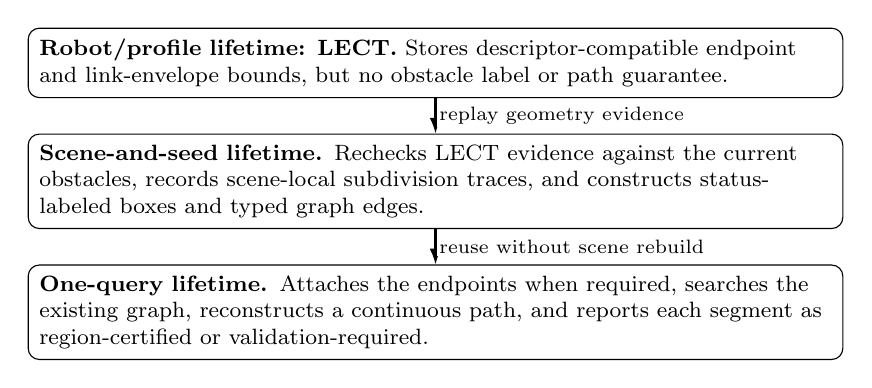
\begin{tikzpicture}[
  node distance=4.5mm,
  box/.style={draw,rounded corners,align=left,text width=0.83\columnwidth,
              inner sep=4pt,font=\footnotesize},
  flow/.style={-{Latex[length=2mm]},thick},
  label/.style={font=\scriptsize,fill=white,inner sep=1pt}
]
\node[box] (lect) {\textbf{Robot/profile lifetime: LECT.}
Stores descriptor-compatible endpoint and link-envelope bounds, but no obstacle
label or path guarantee.};
\node[box,below=of lect] (scene) {\textbf{Scene-and-seed lifetime.}
Rechecks LECT evidence against the current obstacles, records scene-local
subdivision traces, and constructs status-labeled boxes and typed graph edges.};
\node[box,below=of scene] (query) {\textbf{One-query lifetime.}
Attaches the endpoints when required, searches the existing graph, reconstructs
a continuous path, and reports each segment as region-certified or
validation-required.};
\draw[flow] (lect) -- node[label,right]{replay geometry evidence} (scene);
\draw[flow] (scene) -- node[label,right]{reuse without scene rebuild} (query);
\end{tikzpicture}
\caption{RBF data flow and object lifetimes. Cache replay changes construction
cost but never imports a previous obstacle decision.}
\label{fig:system_overview}
\end{figure}

% ==============================================================================
\section{Related Work}\label{sec:related}

\subsection{Reusable Planning Objects}
Probabilistic roadmaps and LazyPRM reuse vertices, edges, and cached edge
checks~\cite{kavraki1996probabilistic,bohlin2000path,dellin2016unifying}.
RRT-Connect, BIT*, and FMT* are planner families that
construct query-local trees or implicit sample graphs, while OMPL provides
common implementations and benchmarking infrastructure rather than a distinct
planning paradigm~\cite{karaman2011sampling,kuffner2000rrt,gammell2015batch,
gammell2018informed,janson2015fmt,sucan2012ompl,moll2015benchmarking}. These
methods can be strong single-query or anytime planners, but their reusable state
is primarily discrete.

Region-based methods make free-space volume explicit. IRIS-generated regions
combined with GCS optimization provide optimization-ready convex geometry and a
region graph~\cite{deits2015computing,marcucci2023motion,
marcucci2024shortest,amice2022finding,petersen2023growing,
werner2024approximating}. Classical and adaptive subdivision methods similarly
construct searchable free or mixed cells in configuration space
\cite{lozanoperez1983spatial,brooks1985subdivision}. \rbf{} does not claim a
new subdivision topology. Its distinctions are the endpoint-to-link interval
validator, the separation of robot-only envelope evidence from scene labels,
and the aggregation of region and transition guarantees at query time. It uses
axis-aligned boxes and local finite-cover corridors instead of arbitrary convex
cells, trading geometric expressivity for inexpensive replay, adjacency,
relabeling, and local refill. Its intended role is workload-dependent: it adds
reusable volume beyond edge-only methods without claiming the optimization
flexibility of a general convex-region cover.

Scene edits also expose different maintenance units. Dynamic roadmap methods
revalidate affected edges, while subdivision methods relabel affected cells and
convex-region methods reinflate or recertify affected regions. \rbf{} revisits
scene-local boxes and retained mixed domains, replays robot-only envelope
evidence, and reconstructs incident typed edges. This separation keeps scene
relabeling independent of persistent kinematic evidence; \rbf{} does not claim
a new general theory of incremental replanning.

\subsection{Swept-Volume and Interval Bounds}
Swept-volume methods, convex-hull generator bounds, and capsule radius lifts
provide the geometric basis for link-envelope construction
\cite{blackmore1992swept,abdel2006swept,gottschalk1996obbtree,larsen1999fast}.
The Gilbert--Johnson--Keerthi (GJK) distance algorithm, the Flexible
Collision Library (FCL), and interval Denavit--Hartenberg propagation provide
collision and interval-kinematics primitives used in continuous-collision-
detection pipelines \cite{gilbert1988fast,bergen1999gjk,pan2012fcl,moore2009introduction,
jaulin2001applied,snyder1992interval,merlet2004solving,
merlet2009interval}. Redon \etal{} apply related bounds to articulated
continuous collision detection~\cite{redon2004ccd_avatar,redon2005fast_artic};
Taylor-model and safety methods use similar swept-sphere enclosures
\cite{zhang2007taylor,schwarzer2005adaptive,corrales2011ssl}.

The endpoint bound itself is classical. The contribution here is its use as a
reusable joint-box certificate, together with a cache architecture that stores
kinematic evidence without storing stale obstacle outcomes. Trajectory
optimizers such as CHOMP, STOMP, TrajOpt, and GPMP2 remain complementary: they
can refine a route after \rbf{} supplies reusable volumetric context
\cite{ratliff2009chomp,kalakrishnan2011stomp,schulman2014motion,
mukadam2018gpmp2}.

\FloatBarrier
% ==============================================================================
\section{Problem Formulation and Guarantee Semantics}\label{sec:overview_scope}

For a fixed robot and profile descriptor $\delta$, LECT is denoted
$\mathcal{T}_L$. Preprocessing receives $(\calO,\mathcal{S},\delta)$, where the
seed set $\mathcal{S}$ is fixed before timing, and returns scene-local
subdivision traces $\mathcal{T}_F$, a status-labeled box set $\mathcal{F}$, a
typed graph $G$, and retained domains $\mathcal{C}$ for later refinement or
scene repair. All scene labels and graph edges are computed against the current
obstacle set. In the endpoint-conditioned Shelf protocol, $\mathcal{S}$ includes
the declared task endpoints; in the random-scene protocol, $\mathcal{S}$ contains
robot-specific offline anchors and endpoint attachment belongs to the query
stage.

\begin{assumption}[Collision model for certificates]
\label{ass:collision_model}
The certificate model covers workspace-obstacle collision between active rounded
links and $\calO$; joint limits are enforced by requiring each tested region to
lie in $\Q$. Self-collision, attachments, grippers, task regions, dynamic
feasibility, and other constraints require additional validation policies and
cache descriptors. The experiments use active-link versus workspace-obstacle
collision checks.
\end{assumption}

\begin{table}[!t]
\centering
\caption{Object lifetimes and guarantee semantics under
\Cref{ass:collision_model}.}
\label{tab:guarantee_semantics}
\footnotesize
\setlength{\tabcolsep}{2.5pt}
\renewcommand{\arraystretch}{1.06}
\begin{tabular}{@{}M{0.25\columnwidth}M{0.20\columnwidth}M{0.48\columnwidth}@{}}
\toprule
Object or state & Lifetime & Guarantee condition \\
\midrule
LECT record & Robot/profile & Geometry evidence only; no obstacle label or path guarantee is reused. \\
Region-certified box union & Scene and seed set & Every traversed box passes the conservative current-scene test. \\
Finite-cover oriented bounding-box (OBB) corridor & Scene and seed set & Every cover tile passes the same conservative box test. \\
Search-admitted box or transition & Scene and seed set & Validation-required until converted to a certified region. \\
Returned path & One query & Certified iff every segment is certified; otherwise final discrete validation is required. \\
\bottomrule
\end{tabular}
\end{table}

A \emph{region-certified} segment is collision-free under
\Cref{ass:collision_model}. A \emph{validation-required} segment may guide
search but is not reported as successful unless the complete returned path
passes the fixed-step discrete collision check. Shortcutting or simplification
preserves a certificate only when every modified segment remains inside the
certified region; otherwise the path becomes validation-required. The
experiments also apply the discrete check to region-certified paths as a common
cross-check, but that check is not the source of their certificate.

We distinguish the reconstructed path \gammaraw{} from the returned path
\gammafinal{}. The former is assembled from graph regions and stored transition
geometry before simplification. The latter is the path after common
post-processing. A certificate on \gammaraw{} transfers to \gammafinal{} only
when a containment recheck shows that every modified segment remains inside the
certified box or finite-cover corridor union; otherwise the final status is
\StatusV{} even when the raw corridor was \StatusC{}.

% ==============================================================================
\section{Certified Box Validation}\label{sec:link_envelopes}

For a joint region $I\subseteq\Q$, endpoint envelopes $E_k(I)$ bound endpoint
trajectories, and link envelopes $B_\ell(I)$ bound rounded links over the same
region:
\[
I \mapsto \{E_k(I)\} \mapsto \{B_\ell(I)\}.
\]
Axis-aligned \cspace{} boxes are the global forest primitive. Endpoint evidence
becomes a box certificate only after it is lifted to conservative link envelopes
and those envelopes are separated from the current obstacles.

\subsection{Geometric Foundation}\label{sec:rewrite_geom}

Let $C_0$ be a body-frame shape. The rigid transform
$T(q)x=R(q)x+t(q)$ maps a body-frame point $x$ to workspace at configuration
$q$, and $\mathcal{S}_I(C_0)$ denotes the workspace set swept by $C_0$ as $q$
ranges over $I$. Let $\Ball_p(r)$ denote the radius-$r$ ball in the $p$-norm,
and let $\oplus$ denote Minkowski sum. For a capsule
$C=S\oplus\Ball_2(r)$ with zero-radius center segment $S$,
\[
\mathcal{S}_I(C)=\mathcal{S}_I(S)\oplus\Ball_2(r).
\]
For a convex body $P=\operatorname{conv}(v_1,\ldots,v_m)$, conservative outer
bounds $\widehat{\Gamma}_i(I)$ on the vertex trajectories satisfy
\[
\mathcal{S}_I(P)\subseteq
\operatorname{conv}\Bigl(\bigcup_{i=1}^{m}\widehat{\Gamma}_i(I)\Bigr).
\]
A capsule link therefore requires only bounds on its proximal and distal
endpoint trajectories.

\begin{proposition}[Endpoint envelopes induce link interval envelopes]
\label{prop:endpoint_to_link_envelope}
Consider a rounded link $L=[a,b]\oplus\Ball_2(r)$ and a joint interval $I$. If
endpoint envelopes $E_a(I)$ and $E_b(I)$ satisfy
$\Gamma_a(I)\subseteq E_a(I)$ and $\Gamma_b(I)\subseteq E_b(I)$, then
\[
\mathcal{S}_I(L)
\subseteq
\operatorname{conv}\bigl(E_a(I)\cup E_b(I)\bigr)\oplus\Ball_2(r).
\]
Consequently, any conservative outer representation of the right-hand side is a
valid link interval envelope over $I$.
\end{proposition}

\begin{proof}
For each $q\in I$, the moved center segment is the convex hull of the two moved
endpoints. The endpoint inclusions place every such segment inside
$\operatorname{conv}(E_a(I)\cup E_b(I))$. Adding the fixed radius ball then
bounds the swept rounded link.
\end{proof}

\begin{corollary}[Conservative configuration-space box validation]
\label{cor:box_validation}
Let $I\subseteq\Q$ be an axis-aligned \cspace{} box and let
$\{B_\ell(I)\}$ be conservative link interval envelopes for all active rounded
links. If $B_\ell(I)\cap\calO=\emptyset$ for every link $\ell$, then every
configuration $q\in I$ is collision-free under
\Cref{ass:collision_model}.
\end{corollary}

\begin{proof}
By \Cref{prop:endpoint_to_link_envelope}, each link envelope contains the swept
workspace volume of its link over all configurations in $I$. Disjointness from
$\calO$ for every active link therefore excludes workspace-obstacle collision
throughout the box.
\end{proof}

\paragraph{Numerical conservatism}
A certificate requires outward endpoint propagation, radius padding, and
obstacle separation. For link radius $r_\ell$, an axis-aligned bounding-box (AABB) broadphase pads by
$\Ball_\infty(r_\ell)$, which contains the Euclidean lift
$\Ball_2(r_\ell)$. SupportHull/GJK is certificate-capable only with outward
obstacle inflation, explicit margins, and conservative termination tolerances.
Empirical sources remain search filters.

\subsection{Endpoint Interval Envelopes}\label{sec:rewrite_endpoint_env}

For endpoint $k$, let $\Gamma_k(I)$ denote its exact workspace trajectory over
$I$. The basic cache record is an endpoint AABB because it is compact and can be
exported to each link-envelope representation. Interval forward kinematics
(IFK) performs one interval pass; IFK-AA uses affine arithmetic to preserve part
of the trigonometric correlation along the Denavit--Hartenberg chain.
Hierarchical IFK (HIFK) recursively bisects the joint interval and takes hulls of
child endpoint boxes. The split depth, such as HIFK-5, is part of the cache
descriptor.

The implementation also evaluates critical-sample and analytical extrema
sources. Critical sampling probes interval endpoints, midpoints, near-boundary
configurations, and trigonometric turning candidates. The analytical source
solves low-dimensional sinusoidal boundary subproblems. Unless wrapped by an
independent interval-closure argument, these sources are filters rather than
certificate evidence. Table~\ref{tab:mechanism_endpoint} reports their measured
tightness and cost.

\subsection{Link-Envelope Representations}\label{sec:rewrite_link_env}

For a serial-chain capsule link $\ell$ with endpoint records
$E_{\ell-1}(I)$ and $E_\ell(I)$,
$B_\ell(I)=B_\ell^\circ(I)\oplus\mathcal{R}(r_\ell)$, where
$B_\ell^\circ(I)$ bounds the centerline sweep and $\mathcal{R}(r_\ell)$ is the
selected radius lift.

\paragraph{AABB envelope}
The default broadphase wraps the endpoint envelopes and pads by the link radius:
\[
B_\ell(I)=\operatorname{bbox}\bigl(E_{\ell-1}(I)\cup E_\ell(I)\bigr)
\oplus\Ball_\infty(r_\ell).
\]
Segment subdivision may retain a union of padded sub-envelopes when the tighter
representation offsets its storage cost.

\paragraph{Fixed-direction slab envelope}
A $k$-direction discrete oriented polytope stores lower and upper support values
along a fixed direction set. These slabs can reject close obstacle candidates
after the AABB broadphase and before GJK. Their certificate status follows the
conservatism of the endpoint source and separation test.

\paragraph{SupportHull envelope}
SupportHull stores the two endpoint AABBs and the link radius as a compact
support-function record. A fixed-size GJK narrow phase refines candidates that
survive the AABB and optional slab filters. It preserves more directional
structure than one link AABB while sharing the same upstream endpoint evidence.
Table~\ref{tab:mechanism_link} compares the measured representation costs.

% ==============================================================================
\section{Lifelong Envelope Cache Tree}\label{sec:lect}

LECT stores robot-specific geometry evidence without storing scene validity. It
is a dynamically grown binary $k$-d tree over $\Q$; each node records its joint
interval, split metadata, endpoint evidence, derived link-envelope evidence,
and residency state. A replayed record is always checked against the current
obstacles before a box is admitted.

\subsection{Descriptor and Split Policy}\label{sec:lect_design}

A record is replay-compatible only when the robot model, endpoint source,
envelope representation, split descriptor, link radii, and active-link set match
the current build. For a parent interval $I$, let $I_d^-$ and $I_d^+$ be the
children obtained by splitting dimension $d$ at its midpoint, and define
\[
\mathcal{V}(I)=\sum_\ell \operatorname{vol}(B_\ell(I)).
\]
One implemented depth-wise schedule selects
\[
d^*=\arg\min_d\max\{\mathcal{V}(I_d^-),\mathcal{V}(I_d^+)\}.
\]
The schedule is deterministic; if its selected dimension is unavailable, the
runtime uses the widest active dimension. Joints that cannot affect any retained
endpoint are excluded from the candidate set.

Planning cells need not materialize every ancestor. Each cell stores its exact
joint interval, split counts, and descriptor fingerprint. On a cache miss, the
runtime materializes that interval under the same descriptor before scene
validation.

\subsection{Replay and Persistence}\label{sec:lect_storage}

Given a joint interval, LECT replays or materializes endpoint evidence, derives
the requested link representation, and invokes the current scene-validation
policy. Parent or child records may tighten materialization, but no replayed
record carries an obstacle label. During tree descent, transient prefix
transforms are reused so unaffected kinematic-chain prefixes are not recomputed.
In the evaluated pipeline, padded AABB tests precede optional slab and
SupportHull/GJK refinement.

Persistence is selective. Endpoint records and useful derived link records are
stored; inexpensive IFK+AABB records can be regenerated. The prewarm pass fills
target leaves and derives ancestor hulls from child evidence. During the fixed
Shelf timing experiment, the replay store is read-only. Random-scene cache
growth is accounted for in the corresponding per-robot profile.

% ==============================================================================
\section{RapidBoxForest Construction}\label{sec:forest}

For each seed $s_j\in\mathcal{S}$, local materialization records a scene-local
subdivision trace $\mathcal{T}_F^{(j)}$. A trace node may reference a compatible
LECT interval and its geometry evidence, but it owns its own scene label, graph
incidence, and update state. The scene forest is the disjoint union
\[
\mathcal{T}_F=\biguplus_j\mathcal{T}_F^{(j)}.
\]
Different traces may therefore share immutable LECT evidence without merging
their scene-local identities. This seed-indexed collection of traces, rather
than the admitted-box set alone, is what the paper calls a \emph{forest}. The
forest is a provenance and maintenance structure; the typed graph $G$ is the
structure searched by a query. Consolidation may replace overlapping boxes from
different traces in $\mathcal{F}$ and $G$, but the resulting region stores the
identifiers of its source traces, so consolidation does not rewrite the
seed-local provenance forest.

\subsection{Forest and Typed Graph}\label{sec:forest_objective}

A box is an axis-aligned joint interval
$B=[l^{(1)},u^{(1)}]\times\cdots\times[l^{(n)},u^{(n)}]\subseteq\Q$.
The scene validator returns
\[
\sigma_{\calO}(B)\in
\{\StatusC,\StatusV,\StatusB,\StatusI\},
\]
where $\StatusC$ denotes a region-certified box, $\StatusV$ a search-admitted
but validation-required box, $\StatusB$ a blocked box, and $\StatusI$ an
inconclusive box. Under a fixed construction budget,
\[
\begin{aligned}
\mathcal{F}_{\mathrm C}&=\{B\mid\sigma_{\calO}(B)=\StatusC\},\\
\mathcal{F}_{\mathrm V}&=\{B\mid\sigma_{\calO}(B)=\StatusV\},\\
\mathcal{F}&=\mathcal{F}_{\mathrm C}\cup\mathcal{F}_{\mathrm V}.
\end{aligned}
\]
Blocked or inconclusive domains selected for later refinement form
$\mathcal{C}$. The reusable scene output is
$(\mathcal{T}_F,\mathcal{F},G,\mathcal{C})$, where $G$ stores box adjacency and
typed auxiliary transitions.

For two boxes
\[
B_i=\prod_{d=1}^{n}[l_i^{(d)},u_i^{(d)}],\qquad
B_j=\prod_{d=1}^{n}[l_j^{(d)},u_j^{(d)}],
\]
let $\varepsilon_c\ge0$ be the connection tolerance. Candidate connectivity
requires
\[
\max\{l_i^{(d)},l_j^{(d)}\}
\le
\min\{u_i^{(d)},u_j^{(d)}\}+\varepsilon_c,
\quad d=1,\ldots,n.
\]
Exact overlap or contact gives a contained box corridor. A positive tolerance
gap remains validation-required until it is converted to a certified region;
otherwise the returned path must pass final discrete validation.

\begin{algorithm}[t]
\caption{Local box materialization around a seed or retained domain.}
\label{alg:ffb_rewrite}
\footnotesize
\begin{algorithmic}[1]
\REQUIRE Target or witness $q$; optional exact domain $I_0\ni q$; LECT tree
$\mathcal{T}_L$; obstacles $\calO$; validator $V_{\calO}$; descriptor
$\delta$; depth cap $D_{\max}$
\ENSURE Status-labeled interval with status $\StatusC$ or $\StatusV$, or a
retained failure domain with status $\StatusB$ or $\StatusI$
\STATE $I\leftarrow I_0$ if specified; otherwise choose the root containing $q$
\STATE $d\leftarrow0$
\WHILE{$d\le D_{\max}$}
  \STATE $R\leftarrow\operatorname{ReplayOrMaterialize}(\mathcal{T}_L,I,\delta)$
  \STATE derive active-link envelopes $\{B_\ell(I)\}$ from $R$
  \STATE $s\leftarrow V_{\calO}(\{B_\ell(I)\},\calO)$
  \IF{$s\in\{\StatusC,\StatusV\}$}
    \RETURN $(I,s)$
  \ENDIF
  \IF{$I_0$ is specified or $d=D_{\max}$}
    \RETURN retained domain $(I,s)$
  \ENDIF
  \STATE choose the descriptor split; otherwise use the widest active dimension
  \STATE $I\leftarrow$ the child containing $q$; $d\leftarrow d+1$
\ENDWHILE
\end{algorithmic}
\end{algorithm}

\subsection{Build Pipeline}

Construction has four stages. Local materialization first searches for
status-labeled boxes around the declared seeds. A priority sweep expands anchor
and connector coverage before uncovered frontier volume, using deterministic
tie-breaking. Restricted refinement revisits retained blocked or inconclusive
domains under the configured priority and budget. Finally, consolidation removes
or merges boxes only after the resulting region passes the same validator.

\begin{algorithm}[!t]
\caption{Adaptive forest sweep, refinement, and typed-graph construction.}
\label{alg:leaf_sweep_refine}
\footnotesize
\begin{algorithmic}[1]
\REQUIRE Fixed seed set $\mathcal{S}$; LECT tree $\mathcal{T}_L$; obstacles
$\calO$; validator $V_{\calO}$; descriptor $\delta$; configured priority $\pi$;
allowed transition types $\mathcal{T}_{\mathrm{allow}}$; configured sweep,
refinement, and transition budgets
\ENSURE Scene forest $\mathcal{T}_F$, status-labeled boxes $\mathcal{F}$,
typed graph $G$, retained domains $\mathcal{C}$
\STATE initialize queue $\mathcal{P}$ from $\mathcal{S}$ using $\pi$
\STATE $\mathcal{F}\leftarrow\emptyset$; $G\leftarrow\emptyset$;
$\mathcal{C}\leftarrow\emptyset$
\WHILE{$\mathcal{P}$ is nonempty and the sweep budget remains}
  \STATE pop the highest-priority seed or exact retained domain
  \STATE call Algorithm~\ref{alg:ffb_rewrite}
  \IF{a box $B$ with status $s\in\{\StatusC,\StatusV\}$ is returned}
    \STATE insert $(B,s)$ into its scene-local trace and $\mathcal{F}$
    \STATE connect exact-overlap/contact neighbors in $G$
    \STATE generate candidate types in $\mathcal{T}_{\mathrm{allow}}$ within the
    configured transition budget
    \FOR{each candidate transition $e$}
      \IF{$e$ passes a conservative region test}
        \STATE insert $e$ with status $\StatusC$
      \ELSIF{$e$ passes the declared non-conservative admission filter}
        \STATE insert $e$ with status $\StatusV$
      \ELSE
        \STATE reject $e$ or retain its domain as $\StatusB$/$\StatusI$
      \ENDIF
    \ENDFOR
    \STATE enqueue uncovered adjacent frontier domains in priority order
  \ELSE
    \STATE add the returned $\StatusB$ or $\StatusI$ domain to $\mathcal{C}$
  \ENDIF
\ENDWHILE
\FOR{each retained domain selected by the configured refinement rule}
  \STATE bisect by $\delta$, materialize the selected children exactly, and
  insert only $\StatusC$ or $\StatusV$ boxes
\ENDFOR
\FOR{each merge or redundancy candidate selected by the configured consolidation rule}
  \STATE modify $\mathcal{F}$ only after revalidating the retained region
\ENDFOR
\RETURN $\mathcal{T}_F,\mathcal{F},G,\mathcal{C}$
\end{algorithmic}
\end{algorithm}

The benchmark profile fixes the depth caps, descriptor, validation
resolution, priority policy, neighbor rule, and transition budgets before
evaluation. An exact retained domain is materialized as that cell rather than
replaced by a seed-containing ancestor, and every merge is revalidated before
it changes $\mathcal{F}$. Table~\ref{tab:rbf_fixed_profile} lists the Shelf
controls central to interpreting RQ1--RQ2. All remaining implementation settings
are unchanged across the reported RBF rows. The random-scene study likewise
uses one predefined robot--difficulty profile per row, unchanged across its
queries.

\begin{table*}[!t]
\centering
\caption{Selected Shelf b100 controls used in RQ1--RQ2. Depth values belong
to different hierarchy stages and should not be read as one tree depth. All
reported RBF rows use the same settings unless the ablation name identifies the
changed mechanism.}
\label{tab:rbf_fixed_profile}
\scriptsize
\setlength{\tabcolsep}{3.3pt}
\renewcommand{\arraystretch}{1.05}
\begin{tabular}{@{}L{0.16\textwidth}L{0.37\textwidth}L{0.40\textwidth}@{}}
\toprule
Stage & Configuration & Interpretation \\
\midrule
Persistent LECT / scene sweep & depth-23 replay; leaf depths 8--13; descent cap 64; 100-box Shelf budget; deep-box cap 400 & Robot evidence is replayed read-only; scene labels are recomputed. \\
Local refinement & deep free-box depth 62; start depth 32; 800-ms budget; domain seed/success/attempt caps 3/2/3; validation batch 512; 8 workers & These are scene-local refinement controls, not additional LECT depth. \\
Preprocessing connector & 18~ms per pair; at most 2 pairs per gap; 50,000 RRT iterations; 2,000-ms cap; step 0.5; goal bias 0.2; segment resolution 16; at most 200 bridge boxes; 12 paving steps at depth 62 & Exact overlap/contact is certified directly; other geometry requires conservative corridor conversion for status $\StatusC$. \\
Query attachment & paving depth 52; direct sample step 0.08~rad; 12 forced attempts with offset 3; 1,600 fixed RRT iterations; adaptive repair step 0.08~rad; at most 2 repair subdivisions and 24 repair calls & Shelf endpoints are declared before preprocessing but are attached through the same typed transition rules. \\
Search / acceptance & fixed weighted edge cost; discrete-check resolution 16; maximum step 0.01~rad; 10-ms simplification cap; 8 attempts & The cost ranks candidate routes but does not assign certificate status. Planner time excludes final simplification and the discrete check; path quality is measured after both. \\
\bottomrule
\end{tabular}
\end{table*}

No tolerance, candidate edge type, or collision-library call confers a
certificate by itself. A transition receives status \StatusC{} only after the
conservative region tests in Sections~\ref{sec:link_envelopes} and~\ref{sec:obb_endpoint_env} succeed.

The Shelf seed set contains the fixed task anchors and the declared endpoints of
the five queries. Random-scene preprocessing instead uses robot-specific offline
anchors; each predefined start--goal pair is attached during the timed query.
Both modes reuse one scene representation without per-query reconstruction, but only the
Shelf mode is conditioned on the declared query endpoints.

\begin{figure*}[!t]
\centering
\begin{tabular}{@{}c@{\hspace{5pt}}c@{\hspace{5pt}}c@{}}
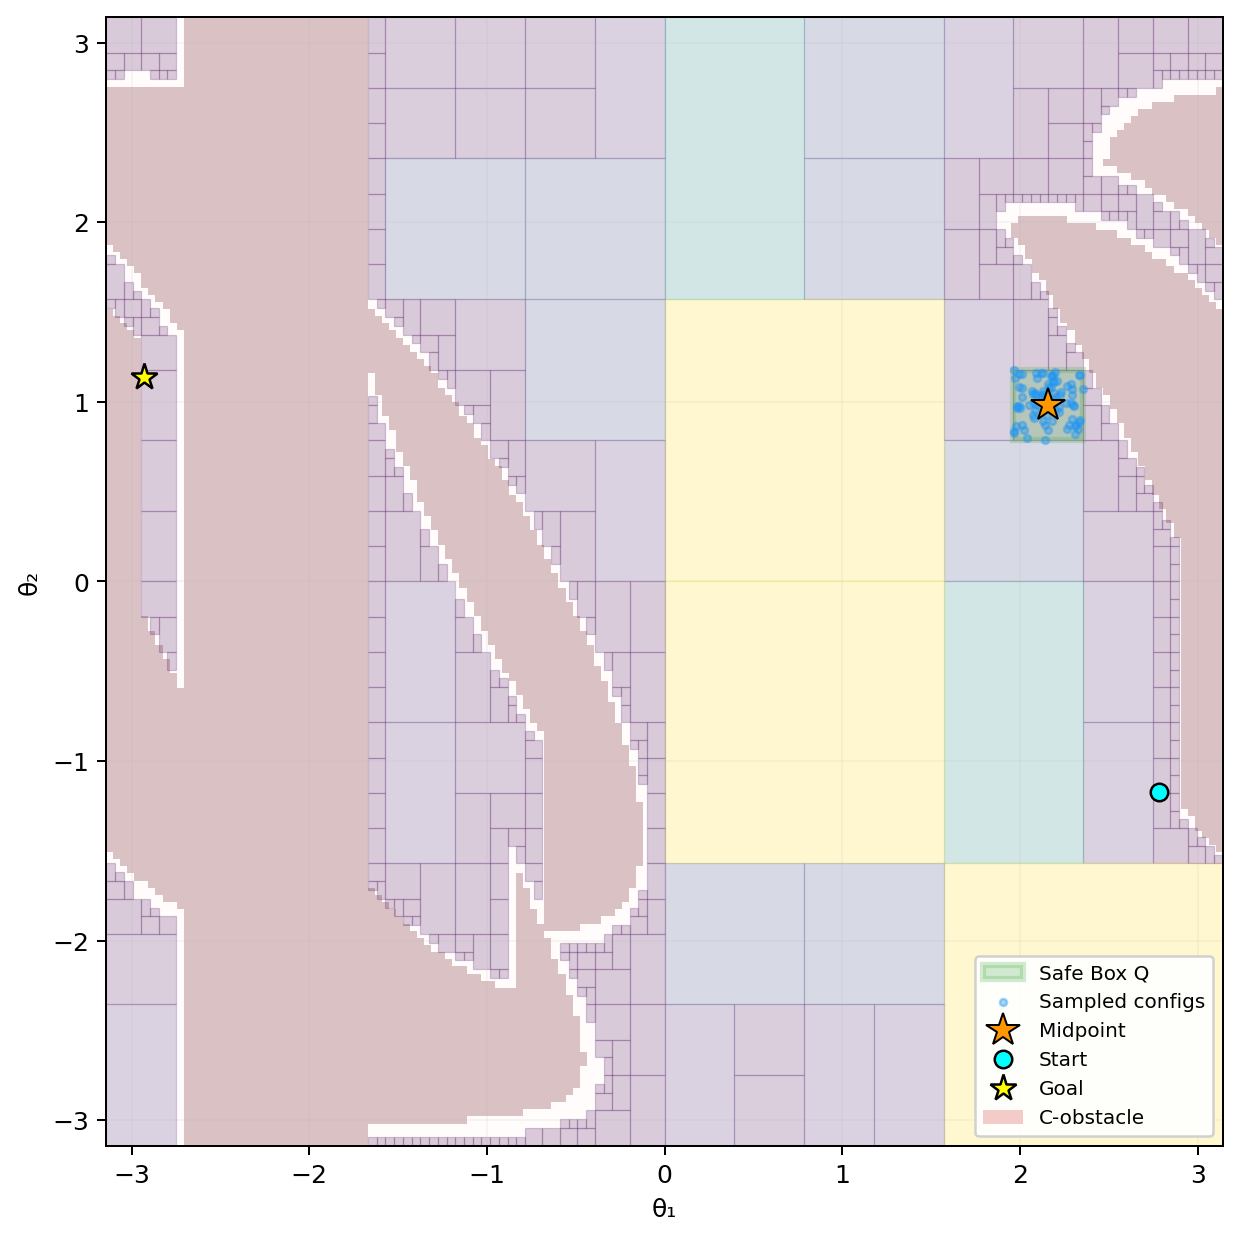
\includegraphics[width=0.30\textwidth]{figures/sbf_grow_1.png} &
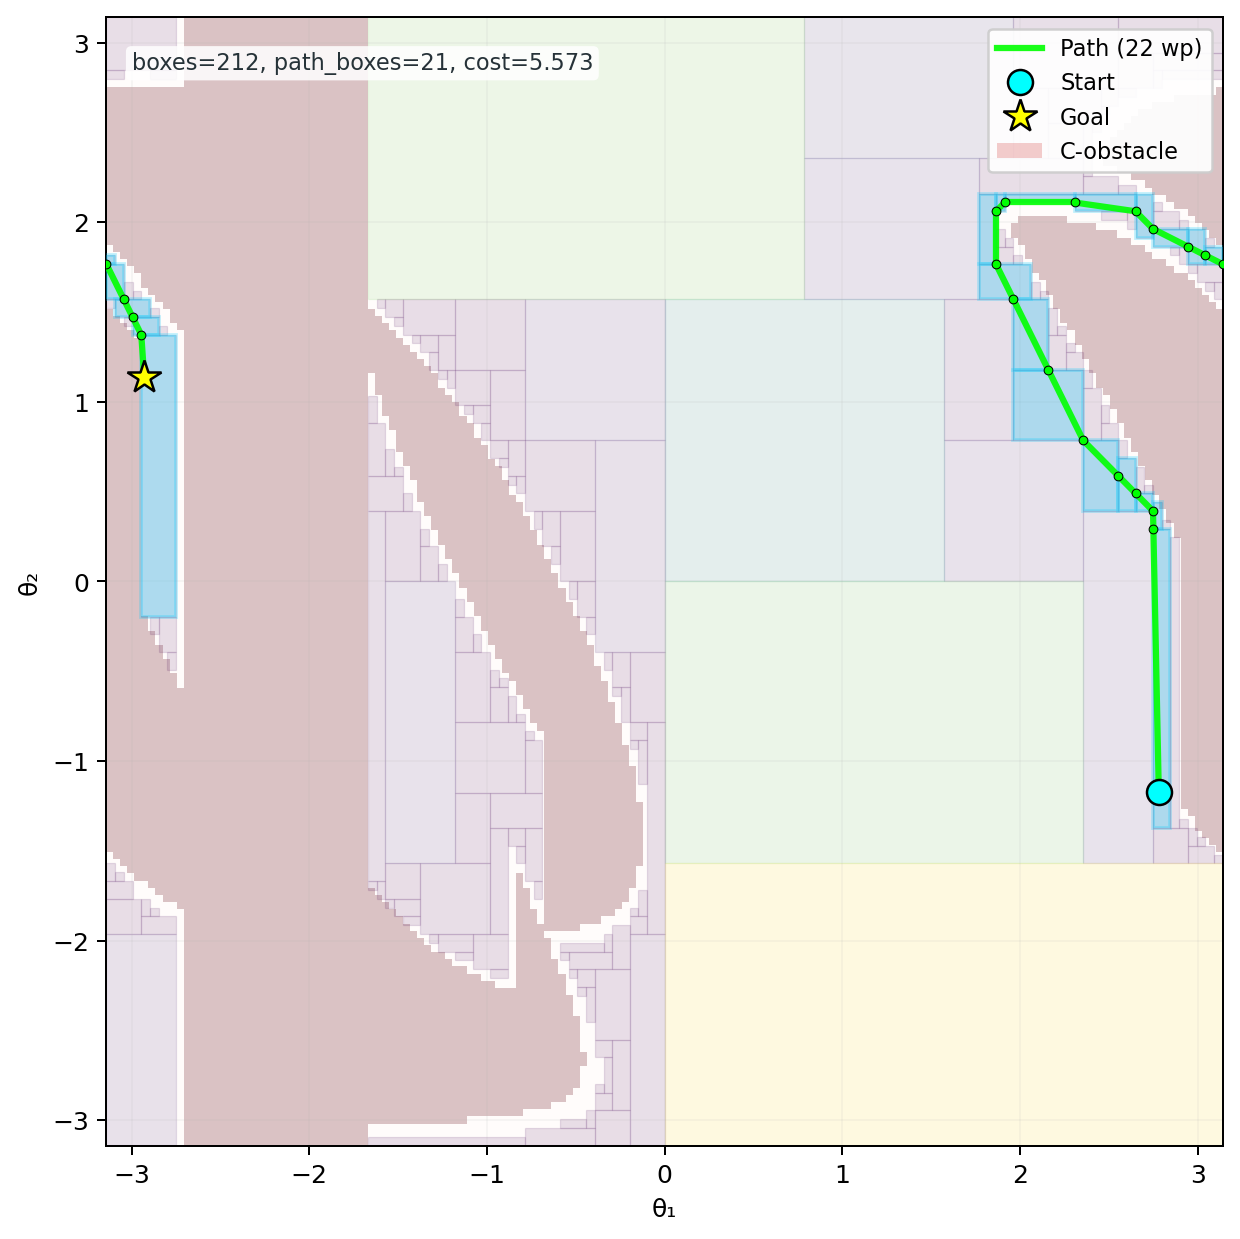
\includegraphics[width=0.30\textwidth]{figures/sbf_grow_3.png} &
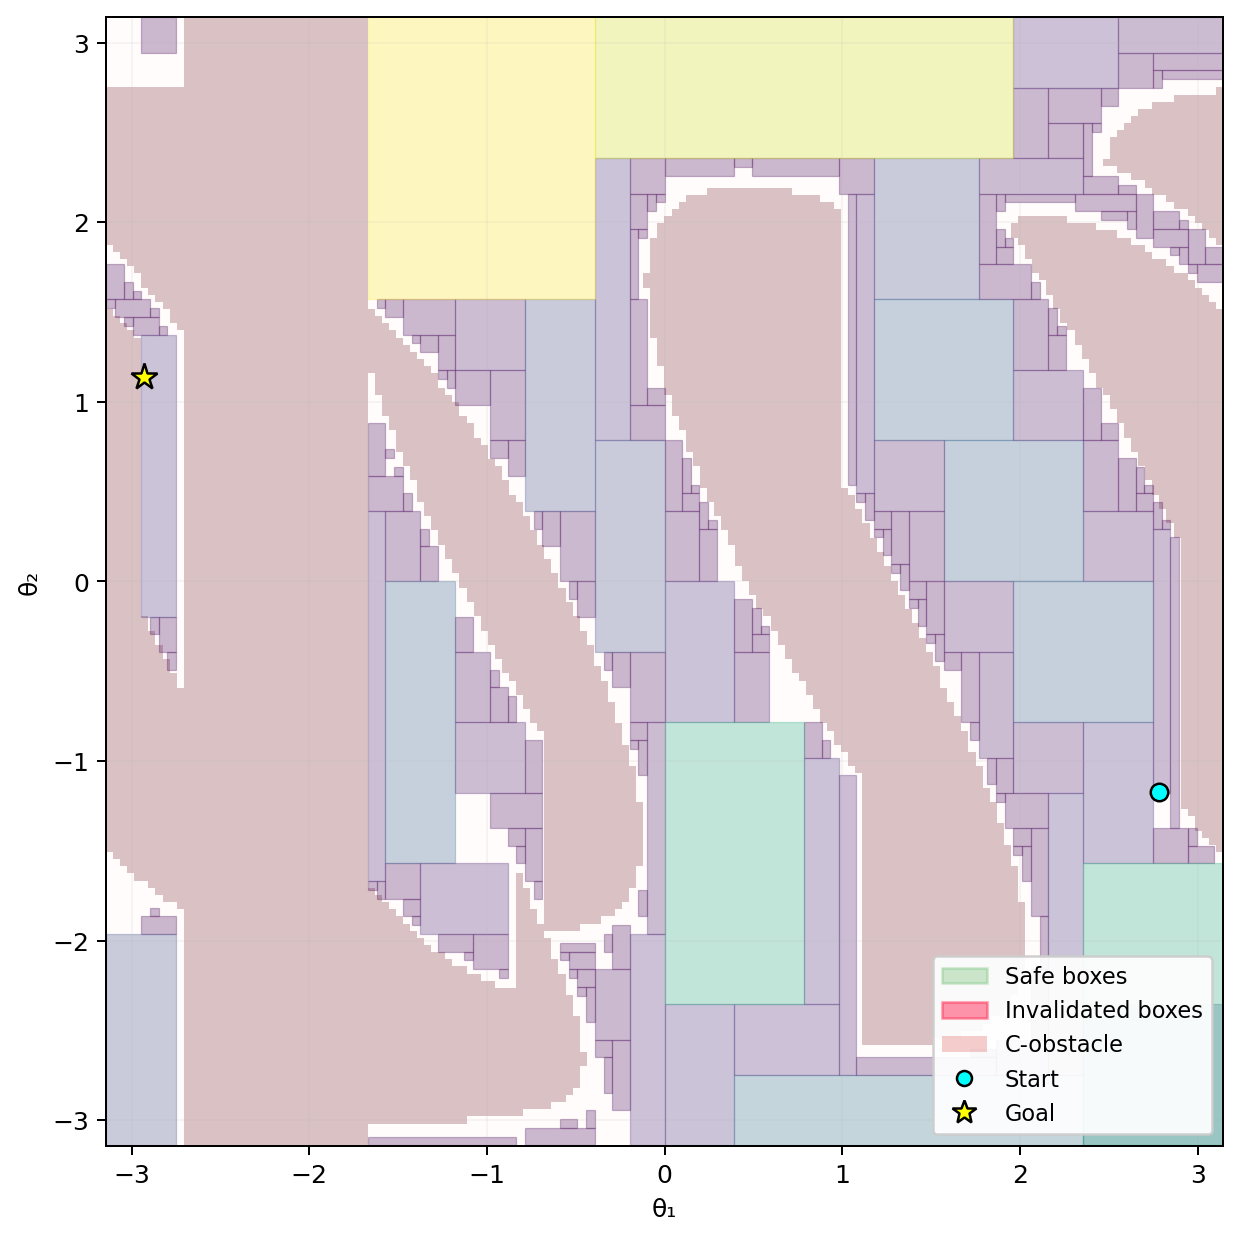
\includegraphics[width=0.30\textwidth]{figures/sbf_grow_6.png} \\
{\footnotesize (a) status-labeled box and local cells} &
{\footnotesize (b) path through the typed graph} &
{\footnotesize (c) local refill after an edit}
\end{tabular}
\caption{Schematic build--query--update cycle. Scene-local traces store
status-labeled \cspace{} boxes, graph search connects them into a corridor,
and an obstacle edit revisits retained local domains before the next query.}
\label{fig:overview}
\end{figure*}

\subsection{Query, Path Reconstruction, and Certificate}

The graph contains overlap/contact edges, tolerance-gap candidates, explicit
segments, finite-cover OBB corridors, and repair witnesses. Edge type describes
how the search connects regions; guarantee status is determined by the backing
region test. Search uses a fixed nonnegative edge cost that combines stored
joint-space path length, a deviation term, and penalties for auxiliary edge
types. The cost profile is fixed before timing within each reported setting.
Cost and guarantee are separate: the cost ranks candidate routes, whereas the
backing region tests determine \StatusC{} or \StatusV{}. Let
$\mathcal{I}_{\mathrm{obb,C}}$ denote all axis-aligned cover tiles belonging to
certified finite-cover OBB corridors, and define the complete certified region
union as
\[
\mathcal{R}_{\mathrm C}
=
\bigcup_{B\in\mathcal{F}_{\mathrm C}} B
\;\cup\!
\bigcup_{I\in\mathcal{I}_{\mathrm{obb,C}}} I.
\]
Algorithm~\ref{alg:query_status} summarizes the query procedure.

\begin{algorithm}[t]
\caption{Query, path reconstruction, and final status aggregation.}
\label{alg:query_status}
\footnotesize
\begin{algorithmic}[1]
\REQUIRE Start $q_s$, goal $q_g$, scene forest $\mathcal{T}_F$, typed graph
$G$, fixed edge-cost function $w$, and current validation policy
\ENSURE Returned path $\gammafinal$ with status $\StatusC$ or $\StatusV$, or failure
\STATE locate containing boxes or configured anchor boxes for $q_s$ and $q_g$
\STATE attach temporary endpoint transitions and assign each status by the same
region rules as the persistent graph
\STATE search $G$ under $w$; return failure if no graph path is found
\STATE for each exact-overlap box pair, select a portal in the box intersection
\STATE concatenate within-box portal segments and stored transition geometry to
obtain $\gammaraw$
\STATE set $\sigma_{\mathrm{raw}}=\StatusC$ iff every raw segment is $\StatusC$;
otherwise set $\sigma_{\mathrm{raw}}=\StatusV$
\STATE apply the configured post-processing to obtain $\gammafinal$
\IF{$\gammafinal=\gammaraw$}
  \STATE $\sigma_{\mathrm{final}}\leftarrow\sigma_{\mathrm{raw}}$
\ELSIF{$\gammafinal([0,1])\subseteq\mathcal{R}_{\mathrm C}$}
  \STATE $\sigma_{\mathrm{final}}\leftarrow\StatusC$
\ELSE
  \STATE $\sigma_{\mathrm{final}}\leftarrow\StatusV$
\ENDIF
\IF{$\sigma_{\mathrm{final}}=\StatusV$ and the final discrete check fails}
  \RETURN failure
\ENDIF
\RETURN $(\gammafinal,\sigma_{\mathrm{final}})$
\end{algorithmic}
\end{algorithm}

Algorithm~\ref{alg:query_status} states the method semantics: a
validation-required output must pass the final discrete check, whereas a
region-certified output derives its guarantee from containment in
$\mathcal{R}_{\mathrm C}$. The experiments additionally apply the same discrete
check to region-certified outputs as a cross-check; failure rejects the run but
does not define the certificate.

\begin{lemma}[Box-corridor certificate]
\label{lem:corridor_certificate}
Let $\mathcal{F}_{\mathrm C}$ be a family of boxes that have passed conservative
link-envelope validation against $\calO$, and let
$R_{\mathcal{F}_{\mathrm C}}=\bigcup_{B\in\mathcal{F}_{\mathrm C}}B$. If a
continuous path $\gamma:[0,1]\to\Q$ satisfies
$\gamma([0,1])\subseteq R_{\mathcal{F}_{\mathrm C}}$, then $\gamma$ is
collision-free under \Cref{ass:collision_model}.
\end{lemma}

\begin{proof}
For any $s\in[0,1]$, containment gives a conservatively certified box
$B\in\mathcal{F}_{\mathrm C}$ with $\gamma(s)\in B$.
Corollary~\ref{cor:box_validation} certifies the robot at that configuration.
Since $s$ is arbitrary, the complete path is collision-free.
\end{proof}

\begin{corollary}[Constructive certified box chain]
\label{cor:constructive_box_chain}
Let $B_1,\ldots,B_m\in\mathcal{F}_{\mathrm C}$ be convex boxes with
$q_s\in B_1$, $q_g\in B_m$, and $B_i\cap B_{i+1}\neq\emptyset$ for
$i=1,\ldots,m-1$. Choose any portal $p_i\in B_i\cap B_{i+1}$. The piecewise-
linear path through $q_s,p_1,\ldots,p_{m-1},q_g$, with each consecutive segment
assigned to the corresponding box, is contained in
$\bigcup_{i=1}^{m}B_i$ and is region-certified.
\end{corollary}

\begin{proof}
Each segment joins two points in one convex box and therefore remains in that
box. The complete path is contained in the certified box union, so
\Cref{lem:corridor_certificate} applies.
\end{proof}

The portal construction closes the link between an exact-overlap graph path and
a continuous region-certified path. Tolerance-gap, explicit-segment, and repair
edges do not satisfy this corollary unless they are converted to a conservative
box or finite-cover OBB corridor.

The portal construction certifies \gammaraw{}. If post-processing changes its
geometry, Algorithm~\ref{alg:query_status} assigns the status of
\gammafinal{} only after the final containment test; a certified raw backbone
is not, by itself, a certificate for a modified returned path.

The lemma establishes collision freedom, not coverage or completeness. Finite
depth, axis alignment, conservative overapproximation, and finite bridge and
repair budgets can all exclude feasible paths.

\subsection{Finite-Cover OBB Corridors}\label{sec:obb_endpoint_env}

Bridge and repair motions can exhibit strong local joint correlation. \rbf{}
therefore allows a transition candidate to be represented by a local OBB in
scaled joint coordinates,
\[
R_{\mathrm{obb}}=\{q_c+A\xi\mid \xi\in[-1,1]^{m}\}.
\]
The global forest remains axis-aligned. To certify the transition, the local
cube is tiled into subcubes $X_\tau$, each tile is enclosed by the joint-space
AABB
\[
I_\tau=\operatorname{bbox}_q(q_c+AX_\tau),
\]
and every $I_\tau$ must pass the standard box validator. Then
\[
R_{\mathrm{obb}}\subseteq\bigcup_\tau I_\tau\subseteq\Cfree.
\]
A transition that does not obtain this finite cover remains
validation-required. Appendix~\ref{app:obb_corridor} gives the optional
correlated endpoint representation used to tighten these local tests.

\subsection{Scene Edits}

Obstacle insertion or removal invalidates only scene-level labels. The scene
cache revisits affected status-labeled boxes and retained domains, replays
compatible LECT evidence, and updates incident graph edges. Insertions recheck
and refill invalidated regions; removals revisit blocked or inconclusive domains
that may have become free. The next query uses the updated graph and the same
status rules in Table~\ref{tab:guarantee_semantics}.

% ==============================================================================
\section{Experiments}\label{sec:exp}

The experiments address five research questions: \textbf{RQ1}, whether LECT
replay lowers reusable Shelf build time; \textbf{RQ2}, where the fixed Shelf
profile lies among roadmap, sampling, and convex-region baselines; \textbf{RQ3},
whether the same trade-off persists across robots and scene difficulty;
\textbf{RQ4}, which envelope choices support the default profile; and
\textbf{RQ5}, how much scene-label maintenance is required after a local edit.

\subsection{Protocol and Accounting}

Timings were measured on Ubuntu~22.04 with an Intel i5-12600KF CPU and 31~GiB of
RAM. The benchmark process uses an eight-thread wall-clock cap. \rbf{} and LECT
use their configured parallel workers, while comparison planners use their
standard implementations within the same process-level cap. The measurements
therefore document a matched process policy, not equal core utilization or a
parallel-scaling claim. Scene instances, query sets, random seeds, and profile budgets were fixed
before evaluation.

$\Tbuild$ denotes preprocessing for one scene state and its fixed seed set,
and $\Tquery$ denotes planner-side work for one query after preprocessing.
$\Tquery$ excludes the common final simplification and post-run discrete
collision check. For reuse horizon $K$,
\[
\Tamort{K}=\frac{\Tbuild}{K}+\Tquery.
\]
The corresponding accepted-path latency would be
\[
\Taccepted{K}=\frac{\Tbuild}{K}+\Tquery+\Tsimplify+\Tvalidate.
\]
Because the compact tables do not report $\Tsimplify$ or $\Tvalidate$, they
support planner-time comparisons rather than total-latency rankings. Their path
ratios are computed after the common 0.010-s simplification budget and a
0.01-rad segment check. The main time--quality plots should therefore be read as
planner time versus post-processed path quality. Region-certified paths also
undergo the discrete check as a cross-check, but that check is not the source of
their certificate.

Path length is the polyline length under a robot-specific joint-space
metric held fixed for every method and reference path within that robot. Ratios
are compared only for the same robot and query; the paper does not compare
absolute joint-space lengths across robot models. For query $q$, let
$\mathcal{R}_q$ denote the precomputed reference set of successful paths after
the common simplification and discrete acceptance rule. The normalization length
is
\[
L_{\mathrm{ref}}(q)=\min_{\gamma\in\mathcal{R}_q}L(\gamma).
\]
The reference set is generated before the reported summaries and shared across
methods. Thus no online row defines its own denominator, and $\Lrefq$ is an
empirical best-observed reference rather than an optimality certificate.
$\Lref$ is used when the query index is implicit.

Sampling units are reported at their native level. In RQ1, $\Tbuild$ is
summarized over eight seed-level builds, whereas $\Tquery$ and $L/\Lref$ are
summarized over 40 seed--query runs. The five-query amortized value combines each
seed-level build with its five-query cycle before summarization. In RQ2, each
query is first summarized over seeds 0--7 and the compact point is the median of
the five query-level medians, so it is descriptive rather than a pooled-run
median. For random scenes, $\Tbuild$ is summarized over ten scene builds in each
robot--difficulty row, whereas $\Tquery$ and $L/\Lrefq$ are summarized over the
fixed retained query set after method-independent direct-segment pruning.
Quartiles are computed separately for these sampling units.

Warm-cache rows include compatible LECT lookup and evidence reads. They exclude
snapshot creation or loading, resident memory, and offline precomputation. The
depth-23 Shelf cache contains 16,777,215 records, occupies 12.75~GiB on disk,
and requires 958.079~s to prewarm. These offline costs are reported separately
rather than folded into the short-horizon preprocessing measurements.

\subsection{RQ1: Shelf+IIWA Replay}\label{sec:exp_shelf_iiwa}

\begin{figure}[!t]
  \centering
  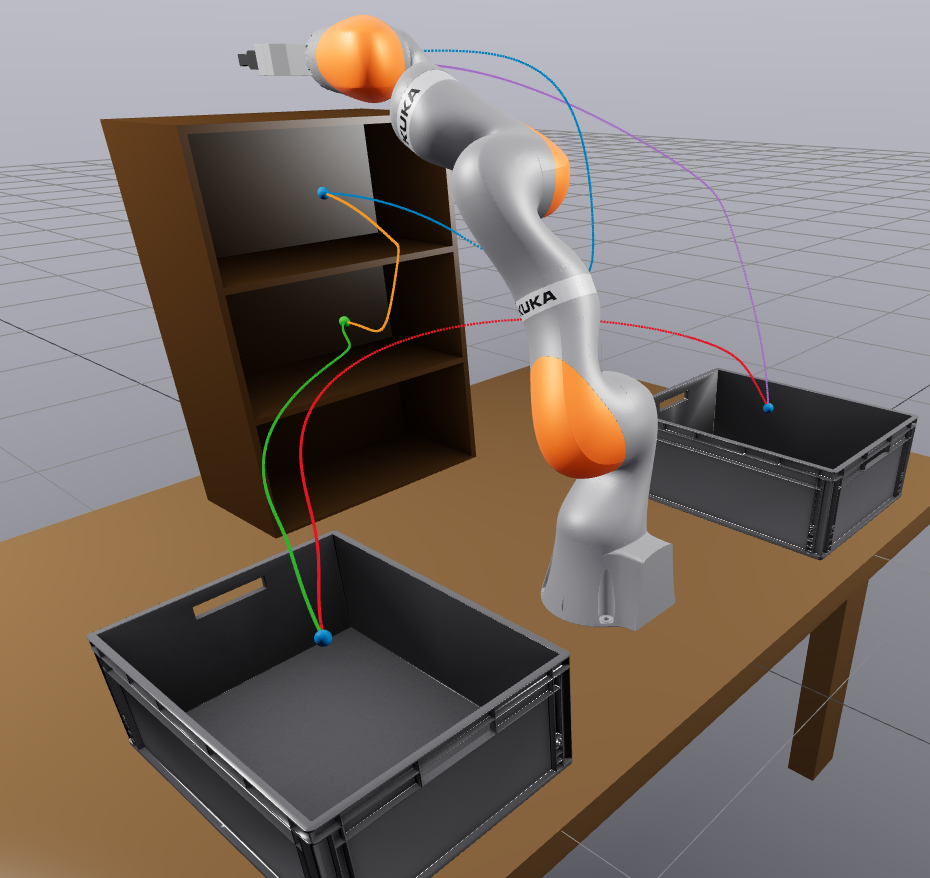
\includegraphics[width=0.94\columnwidth]{figures/Marcucci_scene.png}
  \caption{Fixed Shelf+KUKA LBR iiwa benchmark and five task anchors:
  approach-side (AS), target-shelf (TS), center-shelf (CS), left-bin (LB), and
  right-bin (RB).}
  \label{fig:tro_shelf_scene}
\end{figure}

Figure~\ref{fig:tro_shelf_scene} shows the five-query cycle
AS--TS--CS--LB--RB--AS. These five anchors are the declared query endpoints and
form the seed set before timing. Table~\ref{tab:tro-shelf-ablation}
reports the 100-box Shelf profile (b100) over seeds 0--7.

\begin{table*}[!t]
\centering
\caption{Shelf+IIWA profile and mechanism ablations. $\Tbuild$ is
summarized over eight seed-level builds; $\Tquery$ and $L/\Lref$ use the 40
seed--query runs; $\Tamort{5}$ combines each seed-level build with its
five-query cycle. Times are seconds and entries are median
$[P_{25},P_{75}]$. Planner-time columns describe the raw solve, whereas
$L/\Lref$ is measured on \gammafinal{} after the common post-processing.}
\label{tab:tro-shelf-ablation}
\scriptsize
\setlength{\tabcolsep}{3.2pt}
\renewcommand{\arraystretch}{1.05}
\begin{tabular}{@{}lccccc@{}}
\toprule
Case & $\Tbuild$ & $\Tquery$ & $\Tamort{5}$ & $L/\Lref{}$ & Box-test basis \\
\midrule
RBF baseline & \iqr{0.171}{0.166}{0.174} & \iqr{0.077}{0.072}{0.085} & \iqr{0.111}{0.107}{0.117} & \iqr{1.15}{1.08}{1.39} & Conservative \\
Critical sample$^\dagger$ & \iqr{0.279}{0.275}{0.283} & \iqr{0.087}{0.078}{0.095} & \iqr{0.145}{0.134}{0.151} & \iqr{1.14}{1.09}{1.38} & Filter only \\
Link AABB & \iqr{0.167}{0.164}{0.171} & \iqr{0.083}{0.077}{0.086} & \iqr{0.116}{0.111}{0.119} & \iqr{1.19}{1.08}{1.48} & Conservative \\
Live HIFK-5 & \iqr{2.770}{2.644}{3.003} & \iqr{0.181}{0.139}{0.207} & \iqr{0.739}{0.703}{0.777} & \iqr{1.15}{1.08}{1.43} & Conservative \\
SupportHull only & \iqr{0.193}{0.188}{0.200} & \iqr{0.087}{0.082}{0.095} & \iqr{0.126}{0.120}{0.136} & \iqr{1.15}{1.08}{1.39} & Conservative \\
\bottomrule
\end{tabular}
\par\vspace{0.4ex}
{\scriptsize Box-test basis identifies whether the configured validator can
assign region status $\StatusC$ to a raw corridor before post-processing; it
is not a measured final-path certificate rate. Every reported final path passes
the common 0.01-rad discrete check. $\dagger$ Critical sampling is
non-conservative and is used only as an admission filter.}
\end{table*}

The baseline replays SupportHull link-envelope evidence from the depth-23 cache
and requires 0.171~s to build the reusable scene representation and 0.077~s of
planner time per query. Computing HIFK-5 evidence live under the same depth and
validation budget raises $\Tbuild$ to 2.770~s; its reported median is 16.2
times the replay value. The Link AABB row has a lower reported median build time
together with larger reported median query time and path ratio. These
descriptive intervals are not used for hypothesis testing. Overall, the
results isolate the benefit of replay: the current scene test and final acceptance rule, not the
cache hit, determine the guarantee. Conservative rows can support certified raw
corridors, whereas critical sampling is filter-only; the table does not report
a post-simplification certificate-coverage rate.

\subsection{RQ2: Shelf Fixed-Batch Cross-Algorithm Comparison}
\label{sec:exp_shelf_cross_algorithm}

Table~\ref{tab:tro-shelf-cross-algorithm} and
Fig.~\ref{fig:tro_shelf_cross_tradeoff} summarize the five-query operating
point. The same five queries, 0.01~rad discrete-validation step, 0.010~s
simplification budget, and process-level thread cap are applied to \rbf{},
IRIS-generated regions with GCS optimization, PRM, RRT-Connect, and BIT*. \rbf{}
uses the endpoint-conditioned seed set described in RQ1. The comparison
therefore characterizes a fixed five-query workload rather than endpoint-agnostic
preprocessing. \rbf{}, IRIS/GCS, and PRM report reusable builds; RRT-Connect
and BIT* are invoked independently for each query. BIT* checkpoints are offline quality--time references rather
than online stopping rules.

\begin{table}[!t]
\centering
\caption{Descriptive Shelf operating points summarized over the five
query-level medians. Times are planner-only seconds and exclude the common final
simplification and discrete check; $L/\Lref$ is measured after them.
$\Tamort{5}=\Tbuild/5+\Tquery$. Full query-level intervals are reported in
Appendix~\ref{app:detailed_planning}.}
\label{tab:tro-shelf-cross-algorithm}
\scriptsize
\setlength{\tabcolsep}{3.0pt}
\renewcommand{\arraystretch}{1.04}
\begin{tabular}{@{}lcccc@{}}
\toprule
Method & $\Tbuild$ & $\Tquery$ & $\Tamort{5}$ & $L/\Lref{}$ \\
\midrule
RBF & 0.171 & 0.078 & 0.112 & 1.13 \\
IRIS/GCS & 355.425 & 0.449 & 71.534 & 1.07 \\
PRM & 20.040 & 0.173 & 4.181 & 1.49 \\
RRT-Connect & -- & 0.032 & 0.032 & 2.20 \\
BIT* & -- & 4.004 & 4.004 & 1.03 \\
\bottomrule
\end{tabular}
\end{table}

\begin{figure}[!t]
\centering
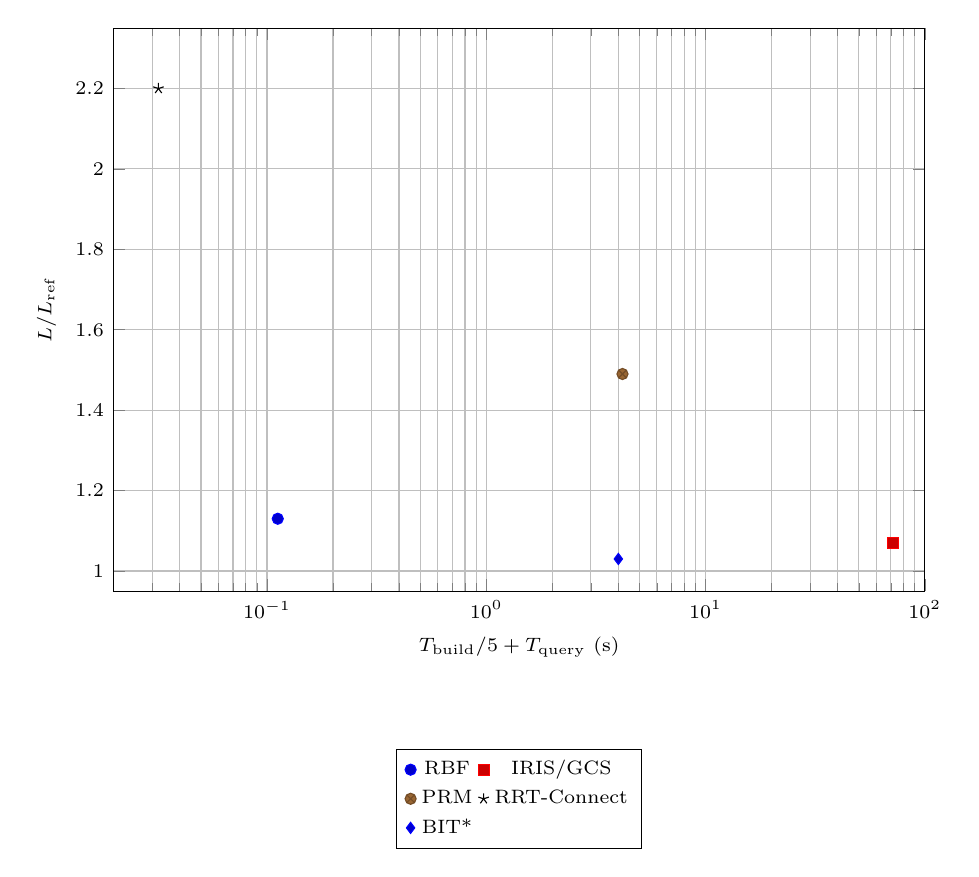
\begin{tikzpicture}
\begin{semilogxaxis}[
  width=0.98\columnwidth,
  height=0.72\columnwidth,
  xlabel={$\Tbuild/5+\Tquery$ (s)},
  ylabel={$L/L_{\mathrm{ref}}$},
  xmin=0.02,xmax=100,
  ymin=0.95,ymax=2.35,
  grid=both,
  legend style={font=\scriptsize,at={(0.5,-0.28)},anchor=north,legend columns=2},
  tick label style={font=\scriptsize},
  label style={font=\scriptsize}
]
\addplot+[only marks] coordinates {(0.112,1.13)}; \addlegendentry{RBF}
\addplot+[only marks] coordinates {(71.534,1.07)}; \addlegendentry{IRIS/GCS}
\addplot+[only marks] coordinates {(4.181,1.49)}; \addlegendentry{PRM}
\addplot+[only marks] coordinates {(0.032,2.20)}; \addlegendentry{RRT-Connect}
\addplot+[only marks] coordinates {(4.004,1.03)}; \addlegendentry{BIT*}
\end{semilogxaxis}
\end{tikzpicture}
\caption{Descriptive Shelf planner-time versus post-processed path-quality
operating points at a five-query reuse horizon. Each point is the median of five query-level medians; no uncertainty bars are shown here, and full intervals appear in
Appendix~\ref{app:detailed_planning}. The horizontal coordinate is planner time
before the separately accounted common post-processing, while the vertical
coordinate is measured after it. Smaller values are better on both axes.}
\label{fig:tro_shelf_cross_tradeoff}
\end{figure}

RRT-Connect has lower $\Tquery$ than \rbf{} in all five queries but
returns longer accepted paths in all five. BIT* returns shorter
paths in all five but requires more planner time. At a five-query horizon,
\rbf{} has a lower reusable build than PRM and IRIS/GCS in this benchmark.
The result is an intermediate operating point for this predefined cycle, not a
universal fastest-query or shortest-path rank.

\subsection{RQ3: Random Multi-Robot Scenes}\label{sec:exp_generalization}

Each fixed benchmark scene contains ten queries shared by every method. Ten seeds
for KUKA LBR iiwa, Universal Robots UR5, and Franka Emika Panda at medium and
hard difficulty yield 600 query instances before pruning. Medium and hard rows
share start--goal pairs; hard rows append a predefined obstacle-prefix
extension. Before any method is summarized, a method-independent rule removes
queries whose direct start--goal segment already passes the common discrete
check. Every displayed method in a robot--difficulty row is evaluated on the
same retained query IDs. The operating-point table is intended as a descriptive
time--quality comparison and does not make a success-rate or completeness claim.

Unlike the endpoint-conditioned Shelf profile, random-scene preprocessing uses
robot-specific offline anchors only. Each start and goal is attached through the
timed query-bridge stage, and the scene representation is not rebuilt. PRM is
built once per scene; RRT-Connect and BIT* are run per query. IRIS/GCS was not
evaluated under the matched random-scene protocol used for this table and is
therefore omitted; it remains part of the matched Shelf comparison.

\begin{table*}[!t]
\centering
\caption{Random-scene operating-point medians. $\Tbuild$ is summarized over ten
scene builds in each row; $\Tquery$ and $L/\Lrefq$ are summarized over the
common retained query runs. Time columns are planner-only seconds before the
common post-processing, whereas path ratios are measured after simplification
and the 0.01-rad discrete check. M/H denote medium/hard, and RRT-C denotes
RRT-Connect. Full $[P_{25},P_{75}]$ intervals are reported in
Appendix~\ref{app:detailed_planning}.}
\label{tab:tro-random-summary}
\scriptsize
\setlength{\tabcolsep}{2.1pt}
\renewcommand{\arraystretch}{1.04}
\begin{tabular}{@{}lccc ccc cc cc@{}}
\toprule
& \multicolumn{3}{c}{RBF} & \multicolumn{3}{c}{PRM} & \multicolumn{2}{c}{RRT-C} & \multicolumn{2}{c}{BIT*} \\
\cmidrule(lr){2-4}\cmidrule(lr){5-7}\cmidrule(lr){8-9}\cmidrule(lr){10-11}
Scenario & $\Tbuild$ & $\Tquery$ & $L/\Lrefq$ & $\Tbuild$ & $\Tquery$ & $L/\Lrefq$ & $\Tquery$ & $L/\Lrefq$ & $\Tquery$ & $L/\Lrefq$ \\
\midrule
IIWA-M & 0.075 & 0.009 & 1.00 & 3.567 & 0.038 & 1.03 & 0.002 & 1.02 & 0.107 & 1.00 \\
IIWA-H & 0.097 & 0.014 & 1.00 & 4.175 & 0.048 & 1.03 & 0.002 & 1.03 & 0.129 & 1.00 \\
UR5-M & 0.262 & 0.075 & 1.05 & 3.124 & 0.323 & 1.02 & 0.023 & 1.23 & 0.134 & 1.01 \\
UR5-H & 0.276 & 0.083 & 1.05 & 2.488 & 0.419 & 1.06 & 0.048 & 1.36 & 0.154 & 1.03 \\
Panda-M & 0.250 & 0.028 & 1.05 & 3.431 & 0.066 & 1.06 & 0.005 & 1.22 & 0.116 & 1.00 \\
Panda-H & 0.224 & 0.043 & 1.05 & 2.337 & 0.054 & 1.10 & 0.056 & 1.25 & 0.164 & 1.01 \\
\bottomrule
\end{tabular}
\par\vspace{0.4ex}
{\scriptsize All displayed methods use the same method-independent
retained query IDs. Every summarized return passes the common discrete check.
RBF uses converted finite-cover OBB-corridor witnesses before post-processing;
this table reports planner time and accepted-path quality rather than a
post-simplification certificate-coverage rate or a success-rate comparison.}
\end{table*}

RRT-Connect has the lowest reported median $\Tquery$ in five of six rows;
\rbf{} is lowest in Panda-Hard. The RRT-Connect median accepted-path ratio is
larger than the \rbf{} ratio in all six rows. Relative to BIT*, \rbf{} has lower
reported median $\Tquery$ in all six; BIT* has a smaller reported median path
ratio in the four UR5/Panda rows, while the displayed two-decimal medians are
equal in the two IIWA rows. These are descriptive operating points, not
significance or equivalence claims.

\subsection{RQ4: Envelope Mechanisms}\label{sec:exp_mechanisms}

Appendix~\ref{app:mechanism_tables} reports descriptive endpoint-source and
link-envelope microbenchmarks over increasing joint-interval widths. They are
used to explain the implementation choices in the default profile rather than
to support population-level statistical claims. IFK-AA and HIFK provide the
conservative endpoint evidence used for box certificates. At a 0.50-rad interval
width, the reported endpoint-volume ratio is 8.61 for IFK-AA and 2.07 for
HIFK-5; HIFK-5 requires 72.32~$\mu$s for endpoint construction in that row.
Critical sampling is faster but undercovers the finite sampled union at larger
widths, while the analytical baseline without interval closure is too
expensive for the hot path and is not itself treated as a certificate. At the link level and the same
0.50-rad width, Link AABB and SupportHull have reported mean volumes of 4.61 and
4.54~m$^3$, but obstacle-test times of 0.790 and 13.026~$\mu$s, respectively.
These descriptive measurements motivate conservative interval evidence, an AABB
broadphase, and selective SupportHull/GJK refinement; they do not constitute a
statistical dominance claim.

\subsection{RQ5: Scene-Edit Maintenance}\label{sec:exp_dynamic_updates}

Table~\ref{tab:tro-dynamic-update} isolates scene-cache maintenance. For each
benchmark edit case, the experiment first builds the 10-obstacle state, adds the
predefined five-obstacle suffix as one batch, builds the 15-obstacle state for the
rebuild reference, and removes that same suffix as one batch. Query search,
bridge construction, simplification, discrete validation, and the next planning
query are excluded.

\begin{table}[!t]
\centering
\caption{Descriptive scene-maintenance time in the fixed edit benchmark,
compared with a warm build of the corresponding target state. Values are
milliseconds, median $[P_{25},P_{75}]$.}
\label{tab:tro-dynamic-update}
\scriptsize
\setlength{\tabcolsep}{3.0pt}
\renewcommand{\arraystretch}{1.05}
\begin{tabular}{@{}lcc@{}}
\toprule
Edit & Maintenance & Target-state warm build \\
\midrule
Add five obstacles, $10\rightarrow15$ & \iqr{6.06}{5.69}{6.54} & \iqr{958.79}{941.67}{1115.18} \\
Remove the same five, $15\rightarrow10$ & \iqr{0.35}{0.31}{1.65} & \iqr{922.75}{897.57}{955.67} \\
\bottomrule
\end{tabular}
\end{table}

Adding the five-obstacle suffix requires 6.06~ms at the median, compared with
958.79~ms for a warm build of the target 15-obstacle state. Removing the same
suffix requires 0.35~ms, compared with 922.75~ms for the target 10-obstacle
state. These values quantify scene-label invalidation, incident-edge updates,
and local-refill bookkeeping only. They do not measure post-edit query success
or accepted-path latency.

\FloatBarrier
\section{Conclusion}\label{sec:conclusion}

RapidBoxForest represents reusable configuration-space regions with
axis-aligned boxes rather than only discrete edges. Conservative endpoint-to-link
envelopes certify whole boxes, LECT amortizes robot-specific kinematic bounds
without retaining stale obstacle labels, and the typed graph exposes whether a
returned segment is region-certified or requires discrete validation. The
representation is built once for a scene state and fixed seed set and is
then reused without per-query scene reconstruction.

After one offline depth-23 precomputation, the endpoint-conditioned Shelf+IIWA
profile preprocesses in 0.171~s rather than 2.770~s with live HIFK-5. Across six
random robot--difficulty rows, RRT-Connect has lower reported median planner
time in five rows but longer median accepted paths in all six. \rbf{} has lower
reported median planner time than BIT* in all six. BIT* has shorter median paths
in four, while the displayed two-decimal median ratios are equal in two.
Adding five obstacles requires 6.06~ms of maintenance at the median, compared
with a 958.79~ms warm build of the target 15-obstacle state; removing the same five requires 0.35~ms, compared
with 922.75~ms for the target 10-obstacle state. These results support box-level
reuse as an intermediate operating point between edge-based roadmaps and more
expressive convex-region covers, not as a universal timing or path-quality rank.

The certificate covers active rounded links against workspace obstacles.
Self-collision, attached objects, grippers, task constraints, dynamic
feasibility, and execution-level limits require additional policies and cache
descriptors. The reported $\Tquery$ excludes final simplification and discrete
validation, and the offline cache prewarm, snapshot, and memory costs are not
included in $\Tbuild$. The Shelf study does not evaluate held-out endpoints that
were unavailable during its endpoint-conditioned preprocessing. The random
study attaches endpoints during the query stage, but it does not test a
distribution shift beyond the fixed benchmark query sets. The experiments
report accepted-path quality after the common discrete check, not a
comprehensive post-simplification C/V coverage rate or per-method
success-rate analysis. The matched random-scene comparison does not include
IRIS/GCS. Finally, finite depth, axis-aligned overapproximation, and finite
bridge and repair budgets make the planner incomplete.

\appendices
\begin{table*}[!t]
\section{Detailed Planning Statistics}\label{app:detailed_planning}
\begin{minipage}{\textwidth}
The main text reports compact operating points. Tables~\ref{tab:tro-shelf-cross-detail}
and~\ref{tab:tro-random-detail} retain the query-level or row-level
$[P_{25},P_{75}]$ intervals used in those summaries.
\end{minipage}
\vspace{0.8ex}
\centering
\caption{Detailed Shelf+IIWA query-level comparison. Reusable build times
are 0.171~s (RBF), 355.425~s (IRIS/GCS), and 20.040~s (PRM); RRT-Connect and
BIT* have no reusable build. Planner times exclude the common final
post-processing, whereas path ratios are measured after it. Entries are median
$[P_{25},P_{75}]$ over seeds 0--7.}
\label{tab:tro-shelf-cross-detail}
\footnotesize
\setlength{\tabcolsep}{3.5pt}
\renewcommand{\arraystretch}{1.03}
\textbf{(a) Per-query planner time $\Tquery$ (s)}\\[0.4ex]
\begin{tabular}{@{}lccccc@{}}
\toprule
Query & RBF & IRIS/GCS & PRM & RRT-Connect & BIT* \\
\midrule
AS$\to$TS & \iqr{0.065}{0.064}{0.070} & \iqr{0.449}{0.449}{0.449} & \iqr{0.198}{0.147}{0.248} & \iqr{0.034}{0.024}{0.052} & \iqr{4.004}{4.002}{4.004} \\
TS$\to$CS & \iqr{0.085}{0.082}{0.089} & \iqr{0.269}{0.269}{0.269} & \iqr{0.173}{0.118}{0.312} & \iqr{0.054}{0.021}{0.089} & \iqr{10.138}{10.004}{10.386} \\
CS$\to$LB & \iqr{0.073}{0.070}{0.077} & \iqr{0.381}{0.381}{0.381} & \iqr{0.136}{0.120}{0.195} & \iqr{0.032}{0.027}{0.070} & \iqr{7.504}{7.504}{7.725} \\
LB$\to$RB & \iqr{0.078}{0.075}{0.083} & \iqr{0.786}{0.786}{0.786} & \iqr{0.164}{0.091}{0.399} & \iqr{0.001}{0.001}{0.002} & \iqr{1.654}{1.654}{1.654} \\
RB$\to$AS & \iqr{0.081}{0.077}{0.086} & \iqr{0.527}{0.527}{0.527} & \iqr{0.252}{0.096}{0.295} & \iqr{0.001}{0.001}{0.001} & \iqr{0.204}{0.204}{0.204} \\
\bottomrule
\end{tabular}

\vspace{0.9ex}
\textbf{(b) Post-processed, discretely checked path ratio $L/\Lref{}$}\\[0.4ex]
\begin{tabular}{@{}lccccc@{}}
\toprule
Query & RBF & IRIS/GCS & PRM & RRT-Connect & BIT* \\
\midrule
AS$\to$TS & \iqr{1.40}{1.34}{1.65} & \iqr{1.44}{1.44}{1.44} & \iqr{1.61}{1.42}{1.73} & \iqr{2.27}{2.05}{2.72} & \iqr{1.06}{1.02}{1.08} \\
TS$\to$CS & \iqr{1.13}{1.11}{1.14} & \iqr{1.26}{1.26}{1.26} & \iqr{2.99}{2.11}{3.22} & \iqr{3.98}{2.80}{5.09} & \iqr{1.09}{1.04}{1.11} \\
CS$\to$LB & \iqr{1.47}{1.32}{1.82} & \iqr{1.07}{1.07}{1.07} & \iqr{1.49}{1.39}{2.09} & \iqr{2.20}{1.75}{2.51} & \iqr{1.03}{1.01}{1.06} \\
LB$\to$RB & \iqr{1.09}{1.07}{1.22} & \iqr{1.07}{1.07}{1.07} & \iqr{1.18}{1.09}{1.27} & \iqr{1.29}{1.27}{1.32} & \iqr{1.02}{1.02}{1.03} \\
RB$\to$AS & \iqr{1.04}{1.03}{1.05} & \iqr{1.01}{1.01}{1.01} & \iqr{1.23}{1.17}{1.24} & \iqr{1.07}{1.03}{1.10} & \iqr{1.02}{1.01}{1.03} \\
\bottomrule
\end{tabular}
\end{table*}

\begin{table*}[!t]
\centering
\caption{Detailed random-scene operating points. Times are seconds.
$\Tbuild$ intervals are over the ten scene builds in each robot--difficulty row;
$\Tquery$ and path-ratio intervals are over the common retained query runs.
Planner times exclude the common final post-processing, whereas path ratios are
measured after it. Direct-segment successes are pruned before all method
summaries.}
\label{tab:tro-random-detail}
\scriptsize
\setlength{\tabcolsep}{2.7pt}
\renewcommand{\arraystretch}{1.02}
\textbf{(a) Reusable build and per-query planner time}\\[0.3ex]
\resizebox{\textwidth}{!}{%
\begin{tabular}{@{}lcccccc@{}}
\toprule
Scenario & RBF $\Tbuild$ & RBF $\Tquery$ & PRM $\Tbuild$ & PRM $\Tquery$ & RRT-Connect $\Tquery$ & BIT* $\Tquery$ \\
\midrule
IIWA-Medium & \iqr{0.075}{0.058}{0.083} & \iqr{0.009}{0.007}{0.011} & \iqr{3.567}{3.007}{3.933} & \iqr{0.038}{0.014}{0.070} & \iqr{0.002}{0.001}{0.002} & \iqr{0.107}{0.087}{0.154} \\
IIWA-Hard & \iqr{0.097}{0.086}{0.105} & \iqr{0.014}{0.011}{0.015} & \iqr{4.175}{3.408}{5.637} & \iqr{0.048}{0.021}{0.102} & \iqr{0.002}{0.002}{0.003} & \iqr{0.129}{0.097}{0.186} \\
UR5-Medium & \iqr{0.262}{0.254}{0.270} & \iqr{0.075}{0.020}{0.086} & \iqr{3.124}{2.966}{3.418} & \iqr{0.323}{0.085}{0.426} & \iqr{0.023}{0.002}{0.049} & \iqr{0.134}{0.101}{0.167} \\
UR5-Hard & \iqr{0.276}{0.264}{0.284} & \iqr{0.083}{0.043}{0.108} & \iqr{2.488}{2.325}{3.048} & \iqr{0.419}{0.129}{0.437} & \iqr{0.048}{0.008}{0.090} & \iqr{0.154}{0.115}{0.171} \\
Panda-Medium & \iqr{0.250}{0.218}{0.265} & \iqr{0.028}{0.013}{0.039} & \iqr{3.431}{3.364}{4.180} & \iqr{0.066}{0.038}{0.159} & \iqr{0.005}{0.002}{0.011} & \iqr{0.116}{0.092}{0.152} \\
Panda-Hard & \iqr{0.224}{0.221}{0.237} & \iqr{0.043}{0.021}{0.053} & \iqr{2.337}{1.627}{3.978} & \iqr{0.054}{0.034}{0.126} & \iqr{0.056}{0.019}{0.136} & \iqr{0.164}{0.123}{0.214} \\
\bottomrule
\end{tabular}}

\vspace{0.8ex}
\textbf{(b) Post-processed, discretely checked path ratio $L/\Lrefq{}$}\\[0.3ex]
\begin{tabular}{@{}lcccc@{}}
\toprule
Scenario & RBF & PRM & RRT-Connect & BIT* \\
\midrule
IIWA-Medium & \iqr{1.00}{1.00}{1.03} & \iqr{1.03}{1.02}{1.12} & \iqr{1.02}{1.01}{1.05} & \iqr{1.00}{1.00}{1.01} \\
IIWA-Hard & \iqr{1.00}{1.00}{1.03} & \iqr{1.03}{1.02}{1.08} & \iqr{1.03}{1.00}{1.07} & \iqr{1.00}{1.00}{1.01} \\
UR5-Medium & \iqr{1.05}{1.00}{1.14} & \iqr{1.02}{1.00}{1.12} & \iqr{1.23}{1.06}{1.54} & \iqr{1.01}{1.00}{1.08} \\
UR5-Hard & \iqr{1.05}{1.01}{1.14} & \iqr{1.06}{1.01}{1.19} & \iqr{1.36}{1.14}{1.58} & \iqr{1.03}{1.00}{1.13} \\
Panda-Medium & \iqr{1.05}{1.02}{1.09} & \iqr{1.06}{1.03}{1.08} & \iqr{1.22}{1.12}{1.35} & \iqr{1.00}{1.00}{1.00} \\
Panda-Hard & \iqr{1.05}{1.01}{1.16} & \iqr{1.10}{1.05}{1.16} & \iqr{1.25}{1.14}{1.37} & \iqr{1.01}{1.00}{1.09} \\
\bottomrule
\end{tabular}
\end{table*}

\begin{table*}[!t]
\section{Mechanism Measurements}\label{app:mechanism_tables}
\centering
\caption{Descriptive endpoint-envelope measurements over joint-interval side
lengths. Widths are radians. IFK-AA and HIFK are certificate-capable; Critical
sampling and the analytical row are non-certifying baselines unless independently
enclosed. The analytical baseline is an empirical normalization source, not
exact ground truth.}
\label{tab:mechanism_endpoint}
\scriptsize
\setlength{\tabcolsep}{4pt}
\renewcommand{\arraystretch}{1.02}
\textbf{(a) Volume ratio relative to the analytical baseline}\\[0.3ex]
\begin{tabular}{@{}lccccc@{}}
\toprule
Source & 0.02 & 0.10 & 0.20 & 0.30 & 0.50 \\
\midrule
IFK-AA & 1.09 & 1.52 & 2.30 & 3.53 & 8.61 \\
HIFK-3 & 1.04 & 1.22 & 1.51 & 1.89 & 3.12 \\
HIFK-5 & 1.02 & 1.13 & 1.30 & 1.51 & 2.07 \\
Critical sample & 1.00 & 1.00 & 1.00 & 0.99 & 0.98 \\
Analytical & 1.00 & 1.00 & 1.00 & 1.00 & 1.00 \\
\bottomrule
\end{tabular}

\vspace{0.7ex}
\textbf{(b) Endpoint construction time ($\mu$s)}\\[0.3ex]
\begin{tabular}{@{}lccccc@{}}
\toprule
Source & 0.02 & 0.10 & 0.20 & 0.30 & 0.50 \\
\midrule
IFK-AA & 5.48 & 6.45 & 6.58 & 6.81 & 7.35 \\
HIFK-3 & 25.94 & 29.16 & 27.21 & 29.27 & 29.38 \\
HIFK-5 & 70.40 & 73.82 & 73.15 & 75.92 & 72.32 \\
Critical sample & 8.68 & 10.03 & 11.56 & 12.69 & 16.33 \\
Analytical & 6429.96 & 6602.25 & 6800.10 & 6927.12 & 7096.01 \\
\bottomrule
\end{tabular}

\vspace{0.7ex}
\textbf{(c) Sampled-union signed gap (mm)}\\[0.3ex]
\begin{tabular}{@{}lccccc@{}}
\toprule
Source & 0.02 & 0.10 & 0.20 & 0.30 & 0.50 \\
\midrule
Critical sample & -0.05 & -1.17 & -4.53 & -10.77 & -30.97 \\
Analytical & 0.00 & 0.00 & 0.00 & 0.00 & -4.49 \\
\bottomrule
\end{tabular}
\par\vspace{0.45ex}
{\scriptsize The signed gap is measured relative to the finite sampled union:
positive values denote overcoverage of that sampled set and negative values
denote finite-sample undercoverage. It is not a certificate margin.}
\end{table*}

\begin{table*}[!t]
\centering
\caption{Link-envelope representations over joint-interval side lengths. Widths
are radians; volume is mean workspace volume. Build time excludes endpoint
envelope construction. Obstacle-test time uses one common mixed far/local probe pool at every width.}
\label{tab:mechanism_link}
\scriptsize
\setlength{\tabcolsep}{3.5pt}
\renewcommand{\arraystretch}{1.02}
\textbf{(a) Mean workspace volume (m$^3$)}\\[0.3ex]
\begin{tabular}{@{}lcccccc@{}}
\toprule
Envelope & 0.02 & 0.05 & 0.10 & 0.20 & 0.30 & 0.50 \\
\midrule
Link AABB & 0.0136 & 0.0201 & 0.0384 & 0.147 & 0.508 & 4.61 \\
SupportHull & 0.000359 & 0.00266 & 0.0143 & 0.106 & 0.449 & 4.54 \\
\bottomrule
\end{tabular}

\vspace{0.7ex}
\textbf{(b) Representation build time ($\mu$s)}\\[0.3ex]
\begin{tabular}{@{}lcccccc@{}}
\toprule
Envelope & 0.02 & 0.05 & 0.10 & 0.20 & 0.30 & 0.50 \\
\midrule
Link AABB & 0.138 & 0.152 & 0.167 & 0.166 & 0.171 & 0.178 \\
SupportHull & 0.205 & 0.214 & 0.218 & 0.219 & 0.217 & 0.250 \\
\bottomrule
\end{tabular}

\vspace{0.7ex}
\textbf{(c) Obstacle-test time ($\mu$s)}\\[0.3ex]
\begin{tabular}{@{}lcccccc@{}}
\toprule
Envelope & 0.02 & 0.05 & 0.10 & 0.20 & 0.30 & 0.50 \\
\midrule
Link AABB & 0.586 & 0.605 & 0.601 & 0.604 & 0.630 & 0.790 \\
SupportHull & 12.520 & 12.850 & 12.267 & 12.223 & 12.659 & 13.026 \\
\bottomrule
\end{tabular}
\end{table*}

\FloatBarrier
\section{Correlated OBB-Corridor Envelopes}\label{app:obb_corridor}

The finite-cover test in Section~\ref{sec:obb_endpoint_env} can be tightened by
preserving the correlation of local OBB coordinates through forward kinematics.
Let $S\in\Real^{n\times n}$ be a positive diagonal joint-scaling matrix,
$U\in\Real^{n\times m}$ have scaled-metric orthonormal columns, and
$h\in\Real_{\ge0}^m$ be the half-width vector. With
$A=S^{-1}U\operatorname{diag}(h)$ and $\Xi=[-1,1]^{m}$,
\[
R_{\mathrm{obb}}=\{q_c+A\xi\mid\xi\in\Xi\}.
\]
For joint coordinate $j$,
\[
q_j=q_{c,j}+a_j^\top\xi,
\]
where $a_j^\top$ is the $j$th row of $A$. Affine-arithmetic propagation yields
an endpoint record
\[
E_k(R_{\mathrm{obb}})=
c_k+\sum_i g_{k,i}\epsilon_i\oplus[-\rho_k,\rho_k],
\qquad \epsilon_i\in[-1,1].
\]
Equivalently,
\[
E_k(R_{\mathrm{obb}})=
p_k(q_c)+J_k(q_c)A\Xi\oplus[-\rho_k,\rho_k].
\]
A conservative coordinatewise remainder can be obtained from an interval Hessian
bound $H_{k,\mu}$ over $R_{\mathrm{obb}}$:
\[
\rho_{k,\mu}\ge
\frac{1}{2}\sum_{a,b}
\left|\left(A^\top H_{k,\mu}A\right)_{ab}\right|.
\]
Sampled remainders do not support a certificate.

For workspace support direction $d\in\Real^3$, the endpoint support bound is
\[
h_{E_k}(d)=d^\top c_k+\sum_i|d^\top g_{k,i}|
+\sum_{\mu=1}^{3}|d_\mu|\rho_{k,\mu}.
\]
The zero-radius centerline and rounded-link support bounds are
\[
\bar h_\ell^\circ(d)=\max\{h_{E_a}(d),h_{E_b}(d)\},
\qquad
\bar h_\ell(d)=\bar h_\ell^\circ(d)+r_\ell\|d\|_2.
\]
Coordinate-axis queries provide an AABB broadphase, and the same record supplies
SupportHull/GJK refinement. These OBB records remain scene-local edge evidence;
they are not nodes in the persistent dyadic LECT.

\IEEEtriggercmd{\enlargethispage{2\baselineskip}}
\IEEEtriggeratref{43}
\bibliographystyle{IEEEtran}
\bibliography{references}

\end{document}
